% Chapter 3

\chapter{Case Study} % Main chapter title

\label{Chapter2} % For referencing the chapter elsewhere, use \ref{Chapter1} 

\lhead{Chapter 2. \emph{Case Studies}} % This is for the header on each page - perhaps a shortened title

%----------------------------------------------------------------------------------------

\section{General Design Considerations of Senior Population}
Senior center is an active node in the community that supply resources
to senior citizens and provide the community with aging related
knowledge~\cite{Dalsanto2009}. Main services offered at a senior
center include: education on a broad range of topics including health,
art, humanity, nutrition etc., volunteering opportunities,
intergeneration programs, meal plans, health screening, physical
training etc. 

There are several main categories of housing choices for the elderly:
independent living, assisted living facilities, Continuing Care
Retirement Communities (CCRC), nursing homes, and special care
facilities as Alzheimer's care facilities~\cite{JFCS2015}. The main
difference are the degree of care provided. Residents of independent
living communities differ from normal communities mainly in the
demographic sence, i.e. the residents are limited to senior
citizens. Assisted living had 24 hour staff and provide living
services such as meal, laundry and bathing. It is meant for seniors
that are not capable of living independently but are not in need of
heavy medical care. Nursing home are more like hospitals with on site
physicians and nurses that provide high degree of medical care in
addiction to living services. CCRC provides a broad range of services
that covers all the services provided in the housing types above and
may include some dementia care~\cite{JFCS2015}. Due to the awareness
of the negative impact of relocation of seniors especially those with
dementia, the CCRC prototype for senior living is the most suitable in
the current case.

The senior community center under discussion in the current project is
a combined community center and housing for senior citizens. It also
integrates with the university population by providing common space to
the community including university population, some housing units for
newly enrolled faculty members and space for elderly-children common
activities with the children from the children's school or from the
community. These makes the function different from a traditional
senior center setting. The case study in this section focuses more on
the aspect specific to the project, such as the instances with mixed
age groups, affiliated to a university, or a combined facility of
living and research.
 
\section{Elderly and Children Combined Facility}
The battle against age segregation is taking place at many places
around the world. In Europe, the concept of ``multi-generation''
community center and the mix-generation housing becomes active
alternatives for dealing with aging of the
society~\cite{Fromm2015}. Several common approaches exist that
facilitates the connections between different age groups:
multi-generation housing, multi-generation community centers, and
adjacency between elderly housing with kindergarten

\subsection{Multi-generational Housing and Neighborhood Center}
In Europe, ``multi-generational neighborhood centers'' are
alternatives to traditional senior centers that creates
inter-generational connections. Its services expanded from traditional
senior center to include community gathering, pre-school, infant care
~\cite{Fromm2015} and advice center that supports different age
groups~\cite{Smith2014}. 

In Germany, the ``multi-generation housing'' program is a government
funded program, which is also part of the ``aging population
plan''~\cite{Smith2014}. Coupled with the multi-generation housing,
the multi-generation community center (or ``multi-generation meeting
house''~\cite{Smith2014}) acts as a space that assist elderly as well
as other generation. It has several features: 1) community education
that enables sharing of knowledges and skills between different age
groups; 2) open meeting space that acts as the ``public living room''
that brings back the conversation and casual encountering between age
groups 3) ``mutual aid'' create bounds between different age groups by
offering and receiving help~\cite{Smith2014}.

One early example of such multi-generation center is the mothers'
centre in Salzgitter, Germany, was launched in 2006 by Ursula von der
Leyen with the aim of creating opportunities of ``encounter and
contact between young and old''~\cite{Smith2014}. It is a one of the
earliest examples of a combined center for children, the youth,
mothers, the community and the elderly. 

\begin{figure}[htbp]
  \centering
  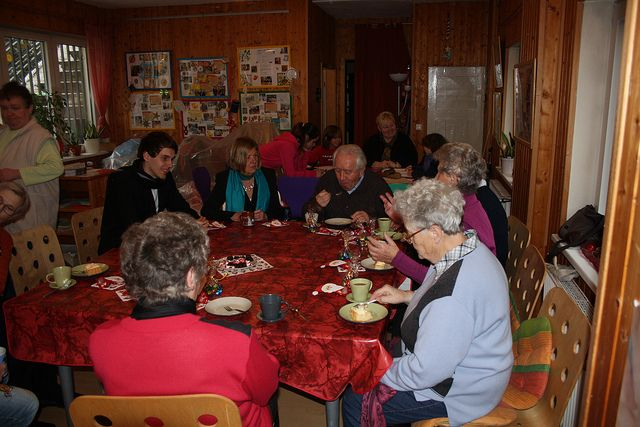
\includegraphics[width=0.7\linewidth]{publicLivingRoom.jpg}
  \caption[Public Living Room]{Public Living Room~\cite{Smith2014}}
  \label{fig:publicLivingRoom}
\end{figure}

\subsection{Mixed-generation Elderly Housing}
In Swabia, Germany, a housing program for elderly was created with 2/3
elderly residents and 1/3 of other age groups. The housing model aims
at helping elderly age in place with helps from other generations in a
``supportive environment''~\cite{Fromm2015}. The common space is
extensible and can hold a variety of activities arranged by social
workers and the residents themselves. The activites take place in the
common space include: morning play of children, affordable lunch for
both the senior residents and people from the neighborhood, informal
community gatherings and rent out space for other community
events~\cite{Fromm2015}.

\subsection{Elderly Housing Next to Kindergarten}
\subsubsection{Altersheim Furttal, A Retirement Home in a Swiss Village}
The retirement home is built near the city center with good public
transportation. This connection provides the residents with a stronger
connection to the society.

There is a kindergarten to the north of the retirement home. The
connections between the two age groups are established with a common
courtyard between the kindergarten and the retirement home. The
interior space design strengthens this connection by arranging a two
story ``lounge space'' adjacent to the common garden.

\begin{figure}
\centering
\begin{subfigure}{0.7\textwidth}
  \centering
  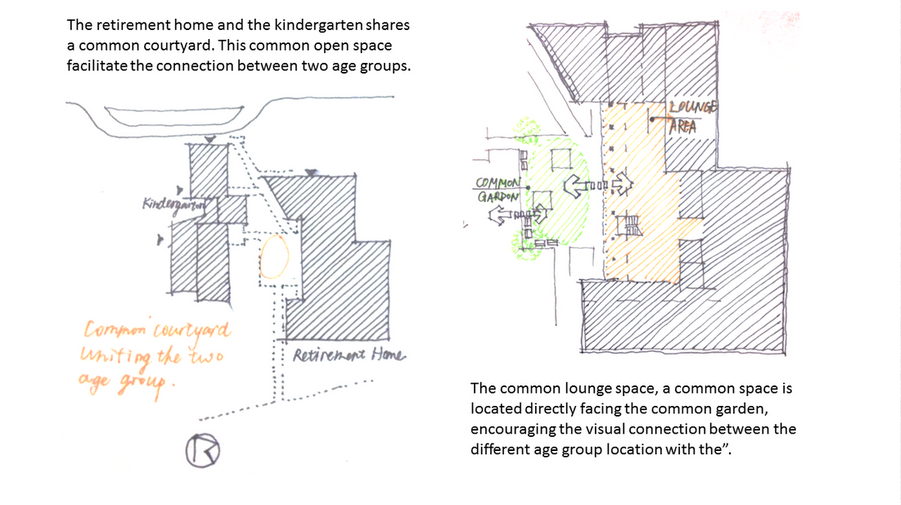
\includegraphics[width=\linewidth]{case1.png}
  \caption{Site Plan Layout of Altersheim Furttal and Kindergarten}
  \label{fig:case1}
\end{subfigure}
\begin{subfigure}{0.7\textwidth}
  \centering
  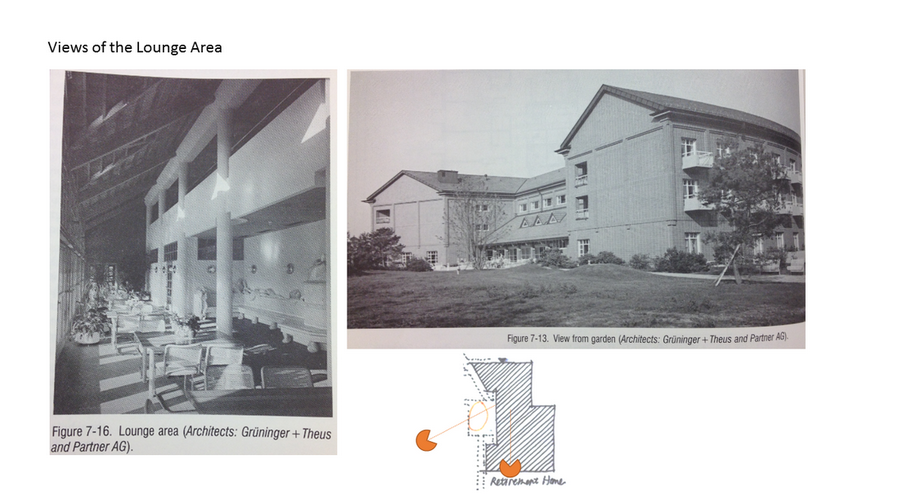
\includegraphics[width=\linewidth]{case2.png}
  \caption{Views of the Lounge Area}
  \label{fig:case2}
\end{subfigure}
\caption{Common Garden and Interior Design in Creating Connections
  between Different Age Groups}
\label{fig:case2}
\end{figure}
\section{University Affiliated Senior Housing}
\subsection{Ithaca College and Longview Partnership}
The Longview project is a combined effort of Ithacca College, Cornell
University and City of Ithaca. It started as an renovation of Tompkins
County Hospital and grow to a CCRC facility providing a variety of
housing choices include independent living, assisted living and
enhanced assisted living.

\subsubsection{Connections between Longview and Ithaca College}
The connections between the Longview program and Ithaca College
include: education opportunities, access to school facilities,
volunteering opportunities and therapy programs supported by students
and staff from related medical programs.

Residents are provided with education opportunities: they have access
to classes taught at Ithaca College or in the Ithaca classroom in
Longview. School facilities such as libraries and gyms are open to
residents to use. School recreational activities are also open for
Longview residents such as sports, art and music events. Students
volunteers participate in the activity arrangement of the Longview
program. Students in the Colloege Physical Therapy and Occupational
Therapy help the staff members give physical traingings to elderly
residents at Longview. This collaboration benefits both the college
students and the staff and elderly residents at Longview. Students
gain parctice experiences and staff and elderlies gain knowledge and
skills for maintaining good physical conditions.

\subsubsection{Site Plan and Building Layout}
Longview community is located to the southwestern of the main campus
of Ithaca College~\cite{googleMapLongiew}. The main apartment building
is a four story building with the main entrance on the third
floor. The layout of the main apartment building includes four living
wings and a common space at the center of each floor. To the north of
the appartment building is the building for enhanced assisted
living. In the west of the site, there are 22 units of duplex
independent living units.
\begin{figure}[htbp]
  \centering
  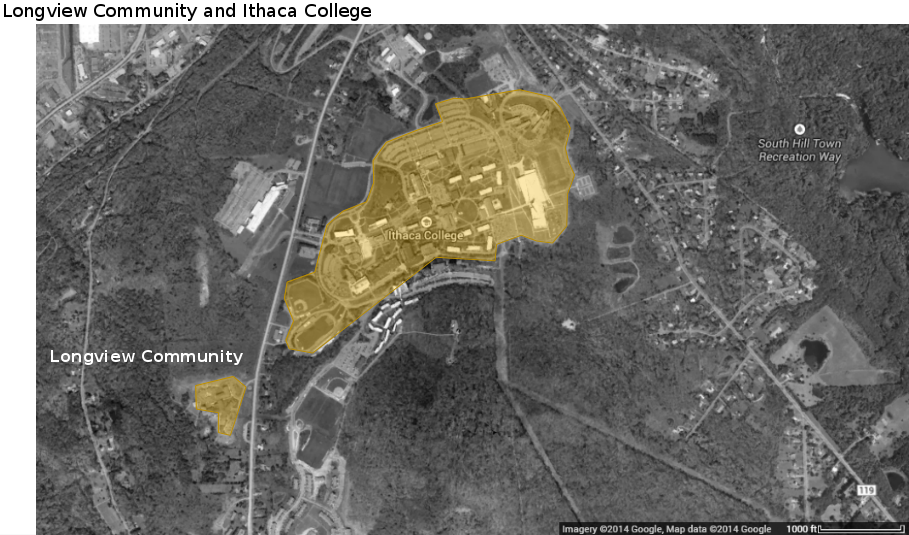
\includegraphics[width=0.7\linewidth]{siteLongview.png}
  \caption[Aerial View of Longview and Ithaca College]{Aerial Longview~\cite{googleMapLongiew}}
  \label{fig:siteLongview}
\end{figure}

\begin{figure}[htbp]
  \centering
  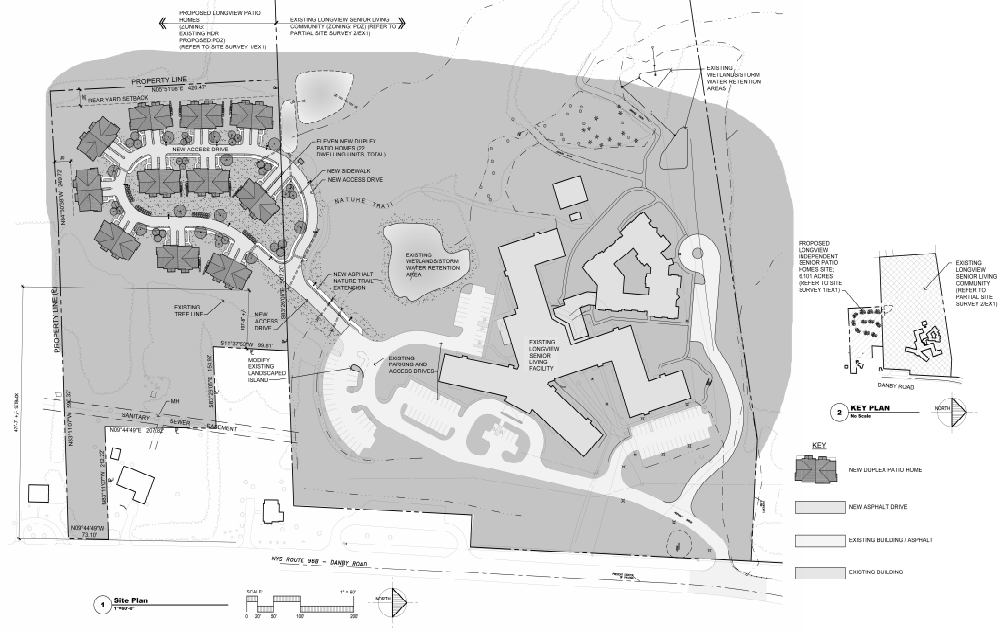
\includegraphics[width=0.7\linewidth]{planLongview.png}
  \caption[Site Plan, Longview]{Site Longview~\cite{patioLongview}}
  \label{fig:planLongview}
\end{figure}

\begin{figure}[htbp]
  \centering
  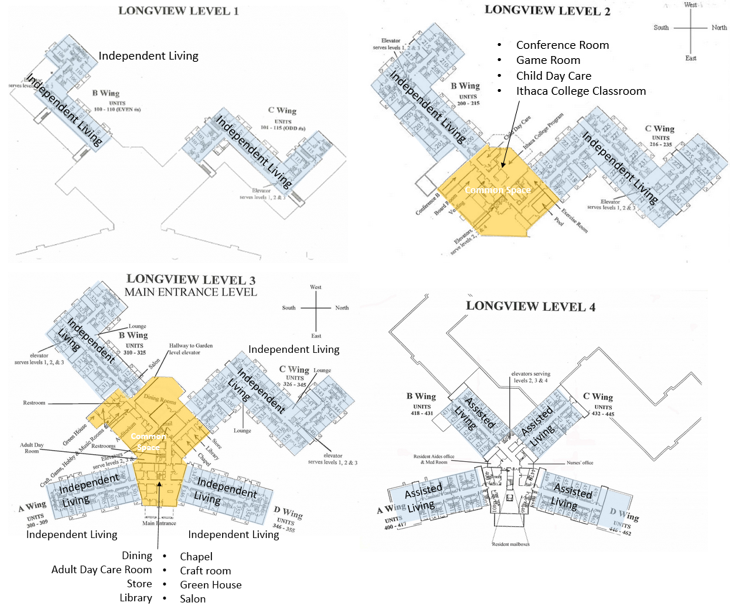
\includegraphics[width=0.7\linewidth]{plan4Longview.png}
  \caption[Building Plan, Longview]{Building Plan
    Longview~\cite{plan4Longview}}
  \label{fig:plan4Longview}
\end{figure}
\subsubsection{Activities}
Activities in Longview includes physical activities, gardening,
intergenerational choir singing etc. As a result of the collaboration
with Ithaca College, residents can take courses and have access to  
the college facilities such as library, gym and art
performances. Recreational facilities in Longview include craft room,
fitness room, game room, green house, library, hair salon, massage
room and walking trail landscape design on the west of the facility.

\subsubsection{Housing Choices and Unit Design}
There are 100 units of independent living appartment units in the
Longview community. The unit types of independent living include small
studio, one-bedroom unit and two-bedroom unit. All three types of
living units include kitchen, bathroom and a balcony. The studio has a
combined living room and bedroom while the other two types have
separate living room and bedroom. The size of studio, single bedroom
and large bedroom are 465 sq.ft., 600 sq.ft. and 858
sq.ft. ~\cite{LongviewIndepend}.
\begin{figure}[htbp]
  \centering
  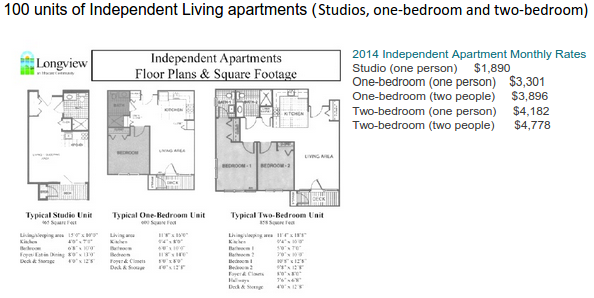
\includegraphics[width=0.7\linewidth]{independUnit.png}
  \caption[Independent Living Unit, Longview]{Independent Living
    Unit, Longview~\cite{LongviewIndepend}}
  \label{fig:independUnit}
\end{figure}

There are also 22 Independent living Patio Homes to the west of the
main appartment building providing high level of living
quality. The Patio unit has a total area of 1355sq.ft. (without
garage)~\cite{LongviewPatio}. Each living unit include two bedrooms ,
two bathrooms: one with shower and the other with bathtub, a living
room, a kitchen, a laundry room, a garage and a patio.
\begin{figure}[htbp]
  \centering
  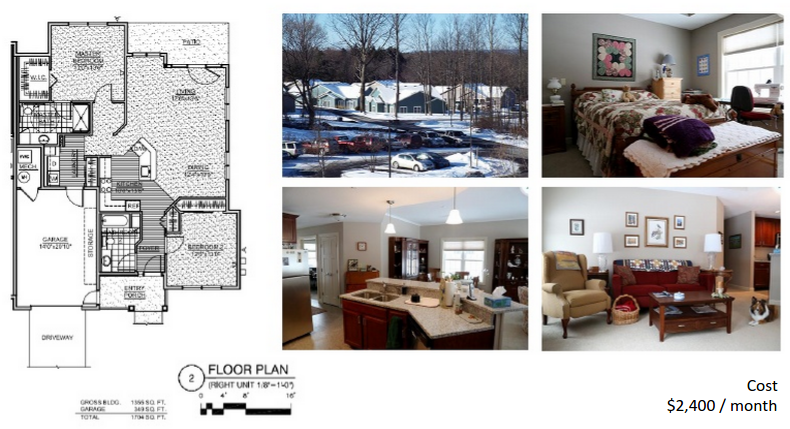
\includegraphics[width=0.7\linewidth]{patioLongview.png}
  \caption[Patio Living Unit, Longview]{Patio Living
    Unit, Longview~\cite{patioLongview}}
  \label{fig:patioLongview}
\end{figure}

There are 60 assisted living units, providing 24-hour assistance, on 
site nurse and emergency pull cords. The assisted living unit is
250sq.ft., smaller than the independent living units. It inlucdes a
bath room, a combined living and sleeping area and a
small refridgerator. No kitchen or balcony is included in the assisted
living units.
\begin{figure}[htbp]
  \centering
  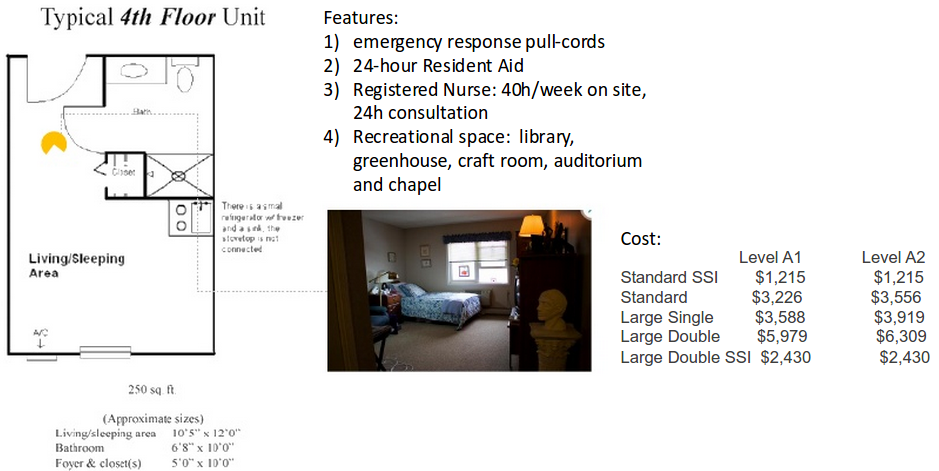
\includegraphics[width=0.7\linewidth]{assistLongview.png}
  \caption[Independent Living Unit, Longview]{Independent Living
    Unit, Longview~\cite{LongviewAssist}}
  \label{fig:assistLongview}
\end{figure}
There are also 24 enhanced assisted living units with additional cares
for residents with memory problems. These units located on the
``Garden Level'' with secure system that monitors exits. Residents
and families also have the option to wear a bracelet sensor for closer
monitoring. The enhanced assisted living units is 220 sq. ft. with the
same function layout as the assisted living units.
\begin{figure}[htbp]
  \centering
  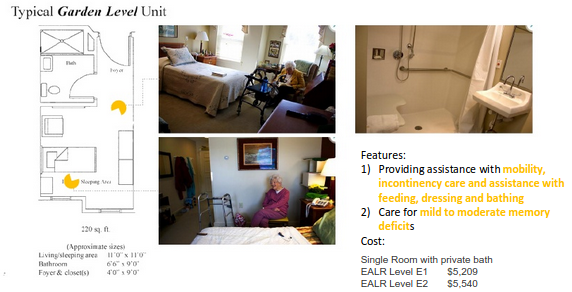
\includegraphics[width=0.7\linewidth]{enhanceLongview.png}
  \caption[Independent Living Unit, Longview]{Independent Living
    Unit, Longview~\cite{enhanceLongview}}
  \label{fig:enhanceLongview}
\end{figure}
\section{Dementia Assisted Living}
\subsection{General Introduction}
``Dementia is an umbrella term for a group of cognitive disorders
typically characterized by memory impairment, as well as marked
difficulty in the domains of language, motor activity, object
recognition, and disturbance of executive function – the ability to
plan, organize, and abstract.''~\cite{CDCdementia} Dementia, or its
most common form Alzheimer, is common in the senior population and
should be considered during the design process of elderly care
facilities. There are 5 million Alzheimer victims in the U.S. and
every 1 out of 3 seniors die in dementia. Women are more vulnerable to
dementia and 2/3 of the Alzheimer victims are
women~\cite{alzorg2014}. This section conduct some related case study
on elderly caring facilities for people with Alzheimer Diseases.

\subsection{Design Features and Concerns for Alzheimer Care}
The physical space acted as a ``therapeutic resource'' in improving
the wellbeing and help reduce the seriousness of
dementia~\cite{Day2000}. Relocation of individual dementia victims to
new environments can increase the possibility of depression and
mortality~\cite{ANTHONY01111987}. This implies the necessity for
dementia dedicated space be incorporated in all categories of senior
housing. If there are not such space in an existing housing program,
when resident develops dementia, they will have to be relocated to
facilities that has dementia care, which might cast negative impact on
the relocated elderly. 

The living unit for cognitively impared people are commonly refered to
as Spetial Care Unit (SCU). The SCU environment have positive impact
on ``communication, self-care, social function and mobility'' status
of dementia victims~\cite{Day2000}. It also reduce emotional strain
and increase satisfactions. The tipical features of a SCU unit
include: less rooms, small room sizes, private rooms and dining space,
access to outdoor environment etc~\cite{Day2000}. Smaller cluster size
showed positive effects on reducing agitation level, aggressiveness,
anxiety and depression~\cite{Day2000}. The positive impact of smaller
cluster group setting also includes relief of stress and negative
attitude of relative care-givers~\cite{Annerstedt19931529, Day2000}.

Special acoustic feature should be added to create a balance between
``sensory overstimulation'' and ``deprivation'', i.e. create a space
that is neither too noisy nor too quiet. Since people with dimentia
tend to also have visual difficulties, the suggested visual
environment is low glare, high contrast and increase lighting
level~\cite{Day2000}. The ``bright light treatment'' showed
improvement on sleep patterns~\cite{Mishima1994}.

For enhancing way-finding, common design suggestions include: provide
views to the outside environment which gives hint of location; create
``landmarks'', large signs; increase lighting level of public spaces
etc. Increase the portion of hallway and reduce the portion of
corridors reduces disorientation~\cite{Day2000}

One of the key features of Alzheimer Care facilities is the living
units should have direct access to enclosed gardens with shaded
porches or trees. Wallking path should form a loop.

The hierarchical pattern of the public to private space transition is
one of the key feature of the cognitively impaired
residents~\cite{seniorLiving}. Private bath and bedrooms are
preferable and the location of public circulation area should be away
from the hallways of private living units. Providing views to the
outside in order to reinforce the day-night rhythms. The activity
groups should be 10-12 persons~\cite{seniorLiving}.

\subsection{Cases}
\subsubsection{Path Design}
One common feature for dementia care facilities is the ``wandering
loop'' structure of path design. The following examples demonstrate
some approaches of such path design.

The partition design of the common space can form a wandering path. In
this community based residential facility, a loop is formed around the
L shaped partition wall. The path connects living room, dining room,
kitchen and activity space (\fref{fig:wander1}).

\begin{figure}[htbp]
  \centering
  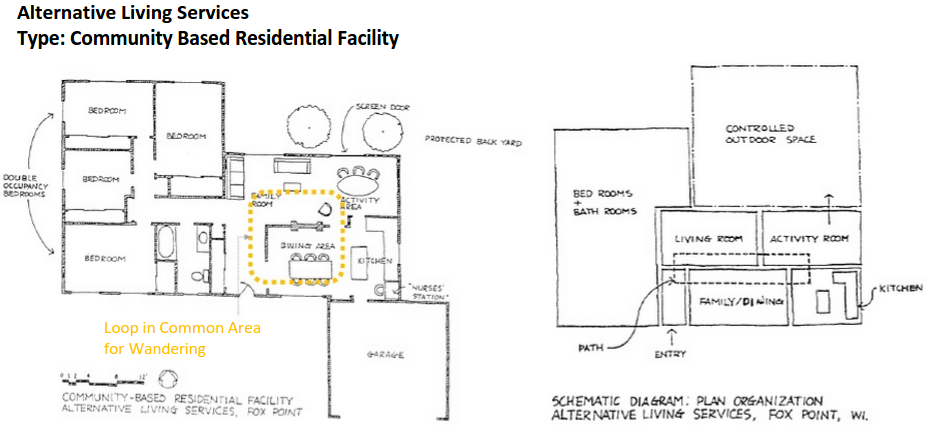
\includegraphics[width=0.7\linewidth]{wander1.png}
  \caption[Wandering Path, Community Based Residential]{Wandering
    Path, community residential~\cite{dementiaCase}}
  \label{fig:wander1}
\end{figure}

The Cedar Lake Home is a free-standing Dementia care facility. The
pavement around the inner garden forms a wondering
path(\fref{fig:wander2}).

\begin{figure}[htbp]
  \centering
  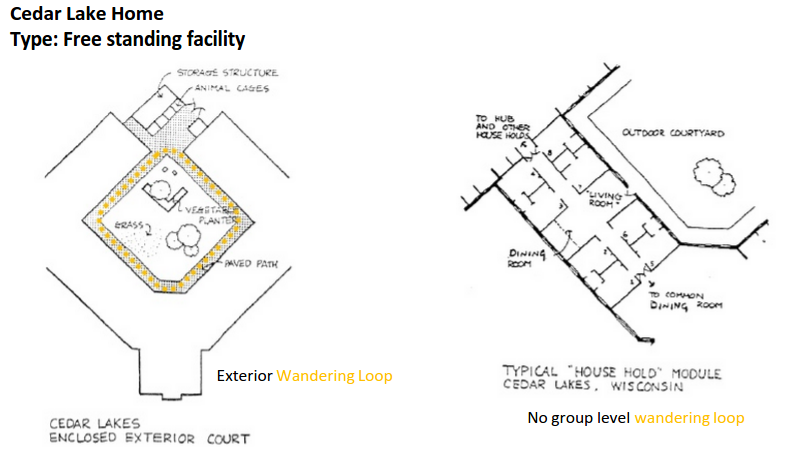
\includegraphics[width=0.7\linewidth]{wander2.png}
  \caption[Wandering Path, Cedar Lake Home]{Wandering Path, Cedar Lake Home~\cite{dementiaCase}}
  \label{fig:wander2}
\end{figure}

The Philadelphia Geriatric Center designs the wandering path with a
different floor covering
\begin{figure}[htbp]
  \centering
  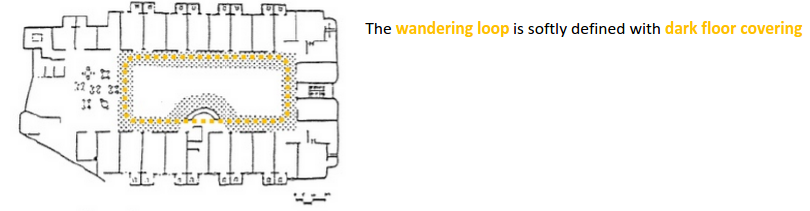
\includegraphics[width=0.7\linewidth]{wander3.png}
  \caption[Wandering Path, Philadelphia Geriatric Center]{Wandering Path, Philadelphia Geriatric Center~\cite{dementiaCase}}
  \label{fig:wander3}
\end{figure}

The Weyauwega Health Care Center has a outdoor garden between two
branches of dementia care housing units. The indoor and outdoor space
together forms a closed-loop wondering path.
\begin{figure}[htbp]
  \centering
  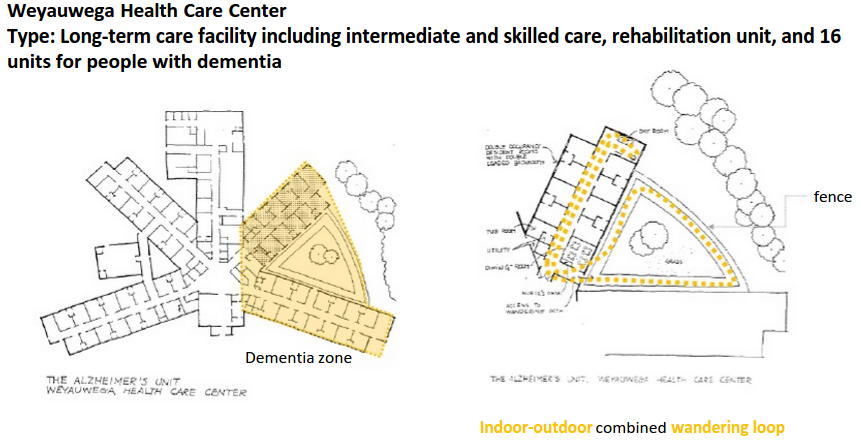
\includegraphics[width=0.7\linewidth]{wander4.png}
  \caption[Wandering Path, Weyauwega Health Care Center]{Weyauwega Health Care Center~\cite{dementiaCase}}
  \label{fig:wander4}
\end{figure}

The John Douglas French Center has a hierarchical common space design
(Left) and a wide wondering path around the center housing units.
\begin{figure}[htbp]
  \centering
  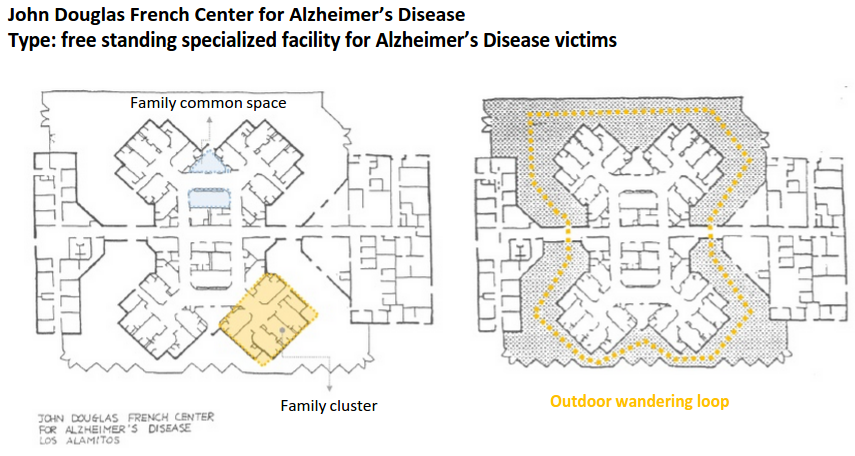
\includegraphics[width=0.7\linewidth]{wander5.png}
  \caption[John Douglas French Center for Alzheimer’s Disease]{John Douglas French Center~\cite{dementiaCase}}
  \label{fig:wander5}
\end{figure}

The Corinne Dolan Center is one of the most frequent appearing example
of Alzheimer's care facilities. It is a research based facility. The
architecture design respond to the special research need by creating a
perfectly symmetrical plan that contains two identical branches. It
facilitates a comparison study between the experiment group and the
control group (\fref{fig:wander6})~\cite{Lewin1990}.

There are two wandering paths, a inner cycle that surrounds the common
area for both branches, and an outer cycle that surrounds the whole
building.
\begin{figure}[htbp]
  \centering
  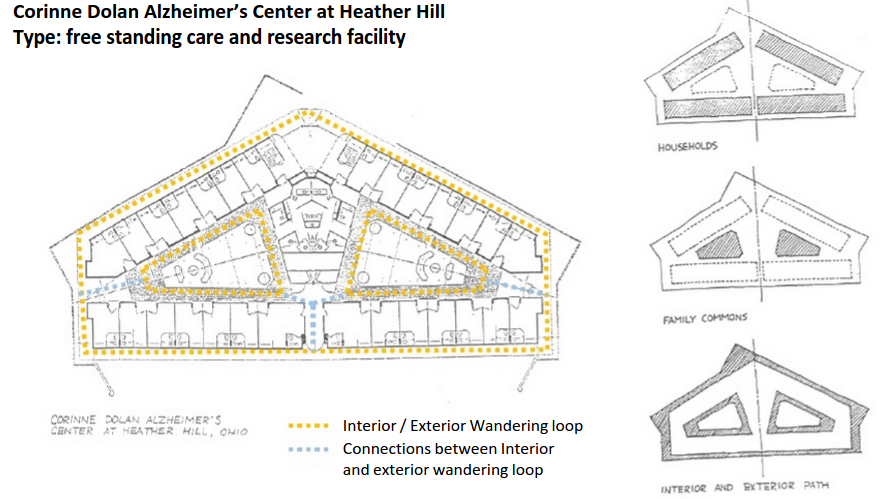
\includegraphics[width=0.7\linewidth]{wander6.png}
  \caption[Corinne Dolan Alzheimer’s Center at Heather Hill]{Corinne Dolan Alzheimer’s Center~\cite{dementiaCase}}
  \label{fig:wander6}
\end{figure}

\subsubsection{Public to Private Space Transition}
The Cedar Lake Home project implemented a hierarchical public space
(\fref{fig:wander2}, \fref{fig:modula}). The adjacent group of eight
living units form a group and share a common space in the center of
the group. The common space of each group joins the garden in the
center of the building. It acts as the next level of common space. The
two X shaped cluster shares a common entrace space (marked as J).
\begin{figure}[h!]
  \centering
  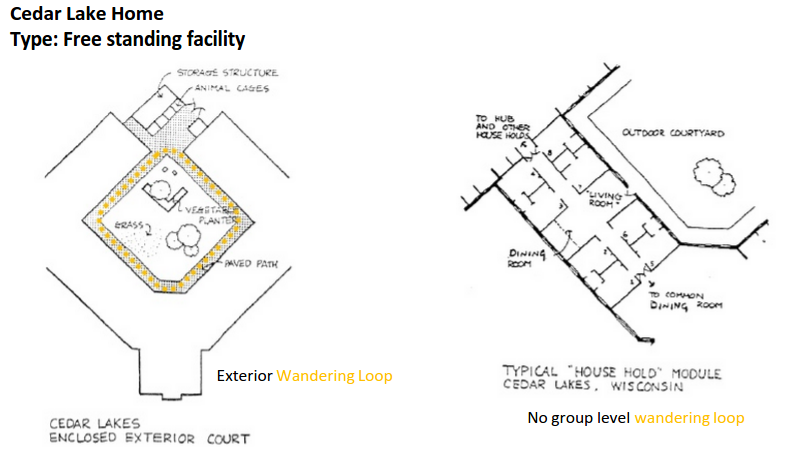
\includegraphics[width=0.7\linewidth]{wander2.png}
  \caption[Hierarchical Public Space, Cedar Lake Home]{Hierarchical
    Public Space, Cedar Lake Home (small scale) ~\cite{dementiaCase}}
  \label{fig:wander2}
\end{figure}
~
\begin{figure}[t]
  \centering
  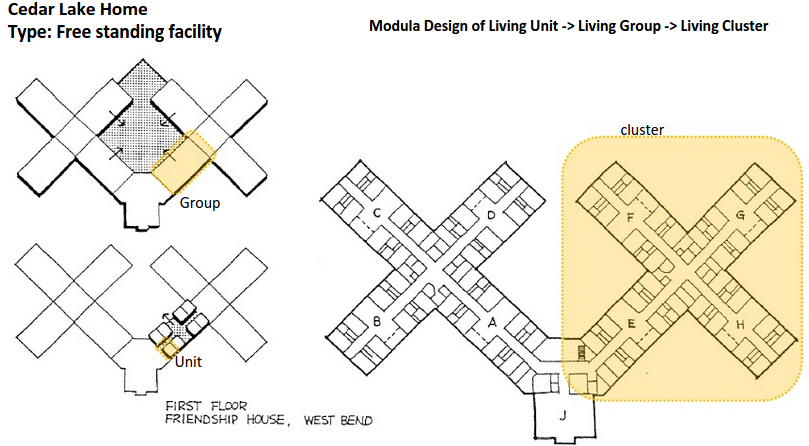
\includegraphics[width=0.7\linewidth]{modula.png}
  \caption[Hierarchical Public Space, Cedar Lake Home]{Hierarchical
    Public Space, Cedar Lake Home (large scale)~\cite{dementiaCase}}
  \label{fig:modula}
\end{figure}
%\section{Sustainable Strategy in Senior Center}